%This fixes a weird error I don't understand
\RequirePackage{ifluatex}
\let\ifluatex\relax

\documentclass[11pt]{article}
\author{Yohan Lefol, Marie Terrien, Alexis Dupis, and Ugo Vidal}
\title{Working Title}

\usepackage{hyperref}
\usepackage{graphicx}
\usepackage{apacite}
\usepackage[margin=3cm]{geometry}
\usepackage{comment}
\usepackage[english]{babel}

\begin{document}
\maketitle

\section{Introduction \label{intro}}
The definition between canonical and non-canonical pathways is not very clear, not does it have a clear cut definition.
We describe canonical pathways as pathways that are well defined in the science field, such as glycolysis. In contrast to this, we define non-canonical pathways as being one or several genes that have an alternate (non-canonical) function which causes them to be a part of a non-standard pathway.

The developed tool can identify non-canonical genes from a gene list. It also has several other applications. The tool allows users to perform a differential gene expression analysis using a negative binomial distribution. In order to do so, the tool implements the DESeq2 R package \cite{love2014moderated}. This aspect of the tool can only be done using COUNT data  from RNA sequencing. Initially this method was selected as it allows users to exploit data from the TCGA (The Cancer Genome Atlas) database, which amasses large quantities of RNAseq files for patients of various cancers.

By pairing this package with our tool, we allow users to identify significant genes from differential analyses and we then look for potential non-canonical genes from the list of isolated significant genes. Additionally, users will have the option to customize MA plots and volcano plots to best suit their publishing needs.

When the tool identifies potential non-canonical genes, the user will be provided with a brief explanation of the canonical pathway that this gene affects along with it's location in the human body, and the same information is given for non-canonical pathways. The tool will also provide any references that have been associated to these genes within our database.

\section{Installation \label{installation}}
\subsection{quick description}
This tool is split into two components, one is the application and processing power, this functional aspect of the tool is downloaded on the users computer and run as a program. The program's interface will then allow users to connect to a database, this database is hosted on the Cellomet website. The database contains all of the information pertaining to non-canonical genes that we have acquired. Once connected to the database, the tool will interact with the users files as indicated by the user and utilize the processing power of the users computer to run the various analyses. This choice was made to prevent a surcharge of a servers processing power, however it is not without consequence.
The DESeq2 package can be heavy on processing power, this is of course dependent on the size of the files given to it. The processing power of a given computer will affect the speed at which analyses are performed.Lastly, as a database connection is required, users must be connected to the internet in order to use the non-canonical analysis aspect of this tool.
\\
This tool also allows users to customize figures based on differential expression data obtained via a DESeq2 analysis, subsequently this allows users to generate customized gene sets based on various parameters. In other words, a user can define his significance parameters and generate both figures and significant gene lists representing these parameters.
\\
Some of the results for the various analyses can be seen in the results tab of the application. All results are automatically downloaded into the users folder of choice. Each result type is described in their respective section of this guide.
\\
Finally, the application contains a section showing how to cite the tool for those who decide to use this tool and it's results.


\subsection{Downloading the tool \label{download_tool}}
Difference MAC and Windows
\subsection{Connecting to the database \label{connect_DB}}
In order to utilize the non-canonical analysis function of this tool, a user must connect to a database (located on Cellomet.com) in order to run the analysis.
To connect to the database, enter the required information. This small survey is used to assess the main uses of this tool along with the type of personnel that utilizes it. This information will be used to better develop the evolution of this tool and cater it to the types of study that appear to need it most.


\section{Non-canonical analysis \label{ncan_analysis}}
This simple analysis is the innovative side of this tool, it is very simple to use. If a user runs a DESeq2 analysis, a non-canonical analysis can automatically be performed on the isolated significant genes, a user must simply check the appropriate box in order to do so. Alternatively, a user can input a gene list file which will be analyzed for non-canonical genes.
The gene list file is very simple in format, it can be seen in \autoref{fig:custom_gene_list}. This file can be created as a text file.
Alternatively, a user can use a DESeq2 significant gene file obtained via the DESeq2 analysis or the data downloaded from custom plots (\autoref{cus_figures}).

\begin{figure}[h!]
\centering
\fbox{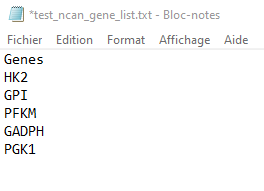
\includegraphics[width=10cm,height=5cm,keepaspectratio]{custom_gene_list.png}}
\caption{An example of a custom gene list}
\label{fig:custom_gene_list}
\end{figure}

The results for this analysis, be it via a custom list or a DESeq2 analysis, is always presented as three separate text files.
\begin{enumerate}
\item non\_canonic\_results.txt
\item canonic\_results.txt
\item references.txt

These files each contain the gene name and gene symbol of identified non-canonical genes in the dataset provided by the user along with information regarding those genes. The information varies based on which file it is contained in.

These text files have been designed to be able to be read by microsoft excel. To do so, a user should open the text file with microsoft excel and select tabs (\textbackslash t) as the separator. This will ensure proper delimitation of the various information contained in the text files.
Also, these results can be viewed within the tool in the results tab. These results are only present after and analysis is done and will not be present if the application is closed or if another analysis is run afterwards. However, files are automatically saved on the users computer, it is not necessary to go through the results tab to save this information.
\end{enumerate}

\section{DESeq2 \label{DESeq2}}
The DESeq2 analysis is a powerfull tool allowing a user to perform differential analyses on large quantities of patient data all while customizing the two conditions of the differential analysis. This type of analysis is very picky about the data type and format used. These are the requirements of the data.
\begin{itemize}
\item The data must be in COUNTS format\\
COUNTS are the basic data format retrieved from an RNA sequencing. COUNTS are the number of \textit{reads} that overlap at a particular genomic position. \textit{Reads} are the oligonucleotides that have been sequenced. In essence, a COUNT is the number of times the mRNA for a specific gene was read.
\item The data format must be as seen in \autoref{fig:data_format_deseq2}.\\
This means that the data must be in csv format, have the gene names as the row headers and patient or sample names as column headers.
CSV files can sometimes be difficult to understand, thus a brief explanation will be given. CSV stands for comma separated vector, this means that a vector (list of elements/values) are separated by commas.


\item Gene names must be in gene symbol format\\
If this section is not respected, a complete DESeq2 analysis will still be performed, however no non-canonic genes will be identified as the data base finds non-canonic genes via their gene symbols. As an example, the data base will not recognize Hexokinase2 as being a non-canonic gene, but it will recognize HK2.
\item Two files must be used, each representing a different condition
This is the basis of the differential analysis, DESeq2 will take in two files with n number of patient genomes. However these files must be split into their respective categories before being inputed into the analysis tool. As an example, one would have a file with all cancer patients between the age of 10 and 50, and a second file for patients of the same cancer but that are between the ages of 70 and 99, This would result in a differential analysis of young vs old.
\end{itemize}
With the two files in the proper format, the user must only select the folder in which he will want to store the results of the analysis. The user will also be able to name his two conditions which will be automatically added to the names of the results created by the analysis. Additionally, a user can choose to create standard MA and Volcano plots, this said, a user will also be able to create custom MA and Volcano plots after a DESeq2 analysis has been finished see section \ref{cus_figures} of this guide.
Before a user can launch an analysis using the non-canonical feature, he will have to connect to the database, this can be done by following the simple steps in the 'Connect to Database' tab of the tool, also talked about in section \ref{connect_DB} of this guide. Otherwise an analysis can be run, however no non-canonical gene analysis will be performed.
Once the analysis has been launched, the user will be prompted to wait until the analysis is over. A notification in the form of a pop up message will be given to user user once the analysis has either finished or if an error has occurred. While the analysis is running, a user should not use the tool and let it work. The user can however continue to use the computer provided the processing power of the computer can handle several tasks at once.
                     
\subsection{Results generated \label{results_DESeq2}}                     
\textbf{THIS SECTION NEXT}
\section{Customizable figures \label{cus_figures}}
This tool allows users to enter differential expression files and create custom MA plots and or custom volcano plots, only a few prerequisites must be met. The differential expression must contain a 'baseMean' and 'padj' columns for MA plots, and a 'padj', 'log2FoldChange', and 'pvalue' columns for volcano plots. Such files are automatically created when a DESeq2 analysis is run, a user must only enter the differential expression file in the file input area of the custom plot.
The customization allows the manipulation of the degrees of significativity for each plot, as in a user can change the degree at which he would like to see the pvalue or padj, the same applies for log2FoldChange.
An important advantage of this is to generate gene lists of varying significance with the customizable volcano plots. By manipulating what padj values and log2FoldChange values are significant, the plot will represent significant genes in a different color, and these genes can then be downloaded with the download data button. In doing so, the user can implement more stringent or lenient significance values on his data set. This gene list can of course then be used for a non-canonical analysis.

Lastly, both custom figure give the option of an alternate color scheme which is deemed more appropriate for color blind or daltonic individuals.


\bibliographystyle{apacite}
\bibliography{references}
\end{document}